\chapter{Inverted Indexing for Text Retrieval}
\label{chapter-indexing}

Web search is the quintessential large-data problem.  Given an
information need expressed as a short query consisting of a few terms,
the system's task is to retrieve relevant web objects (web pages, PDF
documents, PowerPoint slides, etc.) and present them to the user.  How
large is the web?  It is difficult to compute exactly, but even a
conservative estimate would place the size at several tens of billions
of pages, totaling hundreds of terabytes (considering text alone).  In
real-world applications, users demand results quickly from a search
engine---query latencies longer than a few hundred milliseconds will
try a user's patience.  Fulfilling these requirements is quite an
engineering feat, considering the amounts of data involved!

Nearly all retrieval engines for full-text search today rely on a data
structure called an inverted index, which given a term provides access
to the list of documents that contain the term.  In information
retrieval parlance, objects to be retrieved are generically called
``documents'' even though in actuality they may be web pages, PDFs, or
even fragments of code.  Given a user query, the retrieval engine uses
the inverted index to score documents that contain the query terms
with respect to some ranking model, taking into account features such
as term matches, term proximity, attributes of the terms in the
document (e.g., bold, appears in title, etc.), as well as the
hyperlink structure of the documents (e.g.,
PageRank~\cite{Page_etal_1999}, which we'll discuss in
Chapter~\ref{chapter-graphs}, or related metrics such as
HITS~\cite{Kleinberg_JACM1999} and
SALSA~\cite{Lempel_Moran_TOIS2001}).  

The web search problem decomposes into three components:\ gathering
web content (crawling), construction of the inverted index (indexing)
and ranking documents given a query (retrieval).  Crawling and
indexing share similar characteristics and requirements, but these are
very different from retrieval.  Gathering web content and building
inverted indexes are for the most part offline problems.  Both need to
be scalable and efficient, but they do not need to operate in real
time.  Indexing is usually a batch process that runs
periodically:\ the frequency of refreshes and updates is usually
dependent on the design of the crawler.  Some sites (e.g., news
organizations) update their content quite frequently and need to be
visited often; other sites (e.g., government regulations) are
relatively static.  However, even for rapidly changing sites, it is
usually tolerable to have a delay of a few minutes until content is
searchable.  Furthermore, since the amount of content that changes
rapidly is relatively small, running smaller-scale index updates at
greater frequencies is usually an adequate solution.\footnote{Leaving
  aside the problem of searching live data streams such a tweets,
  which requires different techniques and algorithms.} Retrieval, on
the other hand, is an online problem that demands sub-second response
time.  Individual users expect low query latencies, but query
throughput is equally important since a retrieval engine must usually
serve many users concurrently.  Furthermore, query loads are highly
variable, depending on the time of day, and can exhibit ``spikey''
behavior due to special circumstances (e.g., a breaking news event
triggers a large number of searches on the same topic).  On the other
hand, resource consumption for the indexing problem is more
predictable.

A comprehensive treatment of web search is beyond the scope of this
chapter, and even this entire book.  Explicitly recognizing this, we
mostly focus on the problem of inverted indexing, the task most
amenable to solutions in MapReduce.  This chapter begins by first
providing an overview of web crawling
(Section~\ref{chapter-indexing:crawling}) and introducing the basic
structure of an inverted index (Section~\ref{chapter-indexing:intro}).
A baseline inverted indexing algorithm in MapReduce is presented in
Section~\ref{chapter-indexing:index:baseline}.  We point out a
scalability bottleneck in that algorithm, which leads to a revised
version presented in Section~\ref{chapter-indexing:index:revised}.
Index compression is discussed in
Section~\ref{chapter-indexing:index:compression}, which fills in
missing details on building compact index structures.  Since MapReduce
is primarily designed for batch-oriented processing, it does not
provide an adequate solution for the retrieval problem, an issue we
discuss in Section~\ref{chapter-indexing:retrieval}.  The chapter
concludes with a summary and pointers to additional readings.

\section{Web Crawling}
\label{chapter-indexing:crawling}

Before building inverted indexes, we must first acquire the document
collection over which these indexes are to be built.  In academia and
for research purposes, this can be relatively straightforward.
Standard collections for information retrieval research are widely
available for a variety of genres ranging from blogs to newswire text.
For researchers who wish to explore web-scale retrieval, there is the
ClueWeb09 collection that contains one billion web pages in ten
languages (totaling 25 terabytes) crawled by Carnegie Mellon
University in early 2009.\footnote{\texttt{
    http://boston.lti.cs.cmu.edu/Data/clueweb09/}} Obtaining access to
these standard collections is usually as simple as signing an
appropriate data license from the distributor of the collection,
paying a reasonable fee, and arranging for receipt of the
data.\footnote{As an interesting side note, in the 1990s, research
  collections were distributed via postal mail on CD-ROMs, and later,
  on DVDs.  Electronic distribution became common earlier this decade
  for collections below a certain size.  However, many collections
  today are so large that the only practical method of distribution is
  shipping hard drives via postal mail.}

For real-world web search, however, one cannot simply assume that the
collection is already available.  Acquiring web content requires
crawling, which is the process of traversing the web by repeatedly
following hyperlinks and storing downloaded pages for subsequent
processing.  Conceptually, the process is quite simple to
understand:\ we start by populating a queue with a ``seed'' list of
pages.  The crawler downloads pages in the queue, extracts links from
those pages to add to the queue, stores the pages for further
processing, and repeats.  In fact, rudimentary web crawlers can be
written in a few hundred lines of code.

However, effective and efficient web crawling is far more complex.
The following lists a number of issues that real-world crawlers must
contend with:

\begin{itemize}

\item A web crawler must practice good ``etiquette'' and not overload
  web servers.  For example, it is common practice to wait a fixed
  amount of time before repeated requests to the same server.  In
  order to respect these constraints while maintaining good
  throughput, a crawler typically keeps many execution threads running
  in parallel and maintains many TCP connections (perhaps hundreds)
  open at the same time.

\item Since a crawler has finite bandwidth and resources, it must
  prioritize the order in which unvisited pages are downloaded.  Such
  decisions must be made online and in an adversarial environment, in
  the sense that spammers actively create ``link farms'' and ``spider
  traps'' full of spam pages to trick a crawler into overrepresenting
  content from a particular site.

\item Most real-world web crawlers are distributed systems that run on
  clusters of machines, often geographically distributed.  To avoid
  downloading a page multiple times and to ensure data consistency,
  the crawler as a whole needs mechanisms for coordination and
  load-balancing.  It also needs to be robust with respect to machine
  failures, network outages, and errors of various types.

\item Web content changes, but with different frequency depending on
  both the site and the nature of the content.  A web crawler needs to
  learn these update patterns to ensure that content is reasonably
  current.  Getting the right recrawl frequency is tricky:\ too
  frequent means wasted resources, but not frequent enough leads to
  stale content.

\item The web is full of duplicate content.  Examples include multiple
  copies of a popular conference paper, mirrors of frequently-accessed
  sites such as Wikipedia, and newswire content that is often
  duplicated.  The problem is compounded by the fact that most
  repetitious pages are not exact duplicates but near duplicates (that
  is, basically the same page but with different ads, navigation bars,
  etc.)  It is desirable during the crawling process to identify near
  duplicates and select the best exemplar to index.

\item The web is multilingual.  There is no guarantee that pages in
  one language only link to pages in the same language.  For example,
  a professor in Asia may maintain her website in the local language,
  but contain links to publications in English.  Furthermore, many
  pages contain a mix of text in different languages.  Since document
  processing techniques (e.g., tokenization, stemming) differ by
  language, it is important to identify the (dominant) language on a
  page.

\end{itemize}

\noindent The above discussion is not meant to be an exhaustive
enumeration of issues, but rather to give the reader an appreciation
of the complexities involved in this intuitively simple task.  For
more information, see a recent survey on web
crawling~\cite{Olston_Najork_2010}.
Section~\ref{chapter-indexing:summary} provides pointers to additional
readings.

\section{Inverted Indexes}
\label{chapter-indexing:intro}

In its basic form, an inverted index consists of postings lists, one
associated with each term that appears in the collection.\footnote{In
  information retrieval parlance, \emph{term} is preferred over \emph{
    word} since documents are processed (e.g., tokenization and
  stemming) into basic units that are often not words in the
  linguistic sense.} The structure of an inverted index is illustrated
in Figure~\ref{chapter-indexing:inverted-index}.  A postings list is
comprised of individual postings, each of which consists of a document
id and a \emph{payload}---information about occurrences of the term in
the document.  The simplest payload is\ldots nothing!  For simple
boolean retrieval, no additional information is needed in the posting
other than the document id; the existence of the posting itself
indicates that presence of the term in the document.  The most common
payload, however, is term frequency (\emph{tf}), or the number of times
the term occurs in the document.  More complex payloads include
positions of every occurrence of the term in the document (to support
phrase queries and document scoring based on term proximity),
properties of the term (such as if it occurred in the page title or
not, to support document ranking based on notions of importance), or
even the results of additional linguistic processing (for example,
indicating that the term is part of a place name, to support address
searches).  In the web context, anchor text information (text
associated with hyperlinks from other pages to the page in question)
is useful in enriching the representation of document content
(e.g.,~\cite{Metzler_etal_2009}); this information is often stored in
the index as well.

\begin{figure}[t]
\begin{center}
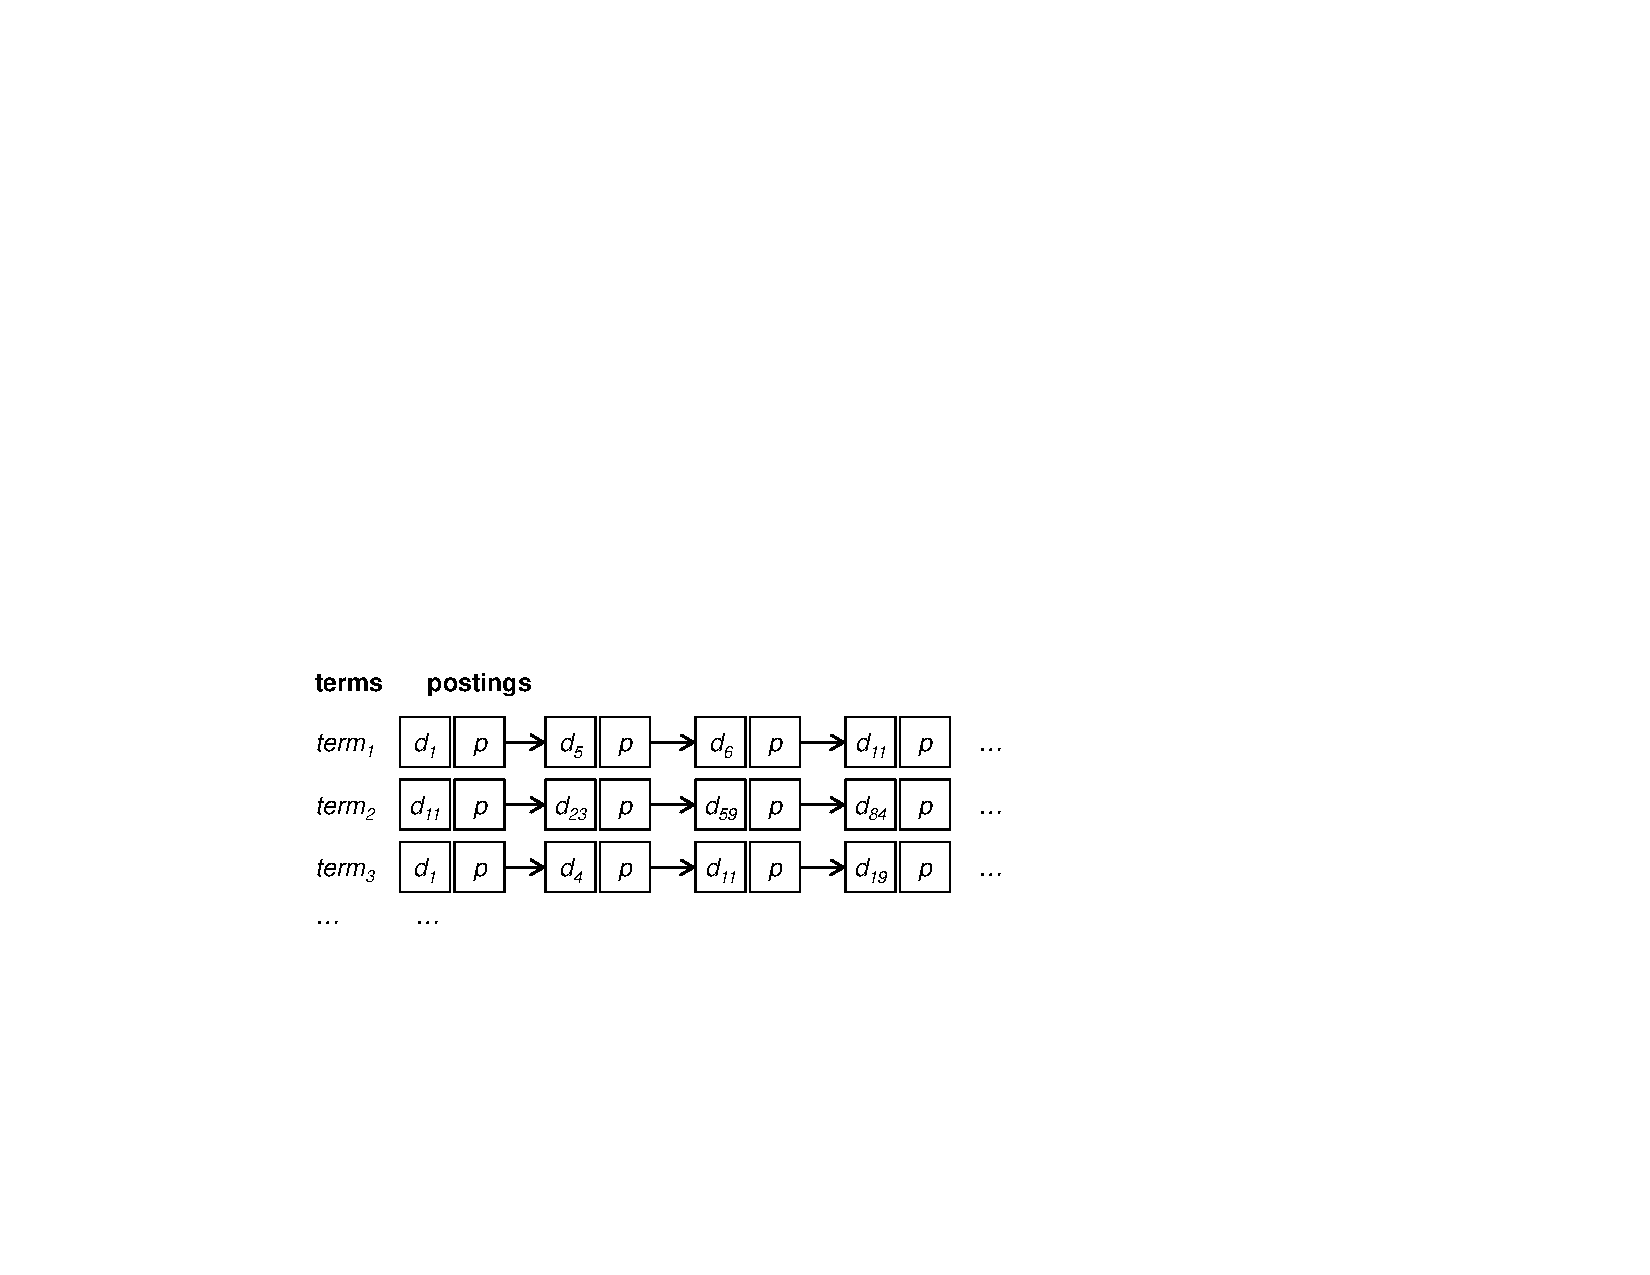
\includegraphics[scale=0.75]{figures/fig-ch4-indexing-inverted-index.pdf}
\end{center}
\caption{Simple illustration of an inverted index.  Each term is
  associated with a list of postings.  Each posting is comprised of a
  document id and a payload, denoted by \emph{p} in this case.  An
  inverted index provides quick access to documents ids that contain a
  term.}
\label{chapter-indexing:inverted-index}
\end{figure}

In the example shown in Figure~\ref{chapter-indexing:inverted-index},
we see that:
\begin{quote}
\emph{term}$_1$ occurs in $\{d_1, d_5, d_6, d_{11}, \ldots\}$, \\
\emph{term}$_2$ occurs in $\{d_{11}, d_{23}, d_{59}, d_{84}, \ldots\}$, and \\
\emph{term}$_3$ occurs in $\{d_1, d_4, d_{11}, d_{19}, \ldots\}$.
\end{quote}

In an actual implementation, we assume that documents can
be identified by a unique integer ranging from 1 to \emph{n}, where
\emph{n} is the total number of documents.\footnote{It is preferable to
  start numbering the documents at one since it is not possible to
  code zero with many common compression schemes used in information
  retrieval; see Section~\ref{chapter-indexing:index:compression}.}
Generally, postings are sorted by document id, although other sort
orders are possible as well.  The document ids have no inherent
semantic meaning, although assignment of numeric ids to documents need
not be arbitrary.  For example, pages from the same domain may be
consecutively numbered.  Or, alternatively, pages that are higher in
quality (based, for example, on PageRank values) might be assigned
smaller numeric values so that they appear toward the front of a
postings list.  Either way, an auxiliary data structure is necessary
to maintain the mapping from integer document ids to some other more
meaningful handle, such as a URL.

Given a query, retrieval involves fetching postings lists associated
with query terms and traversing the postings to compute the result
set.  In the simplest case, boolean retrieval involves set operations
(union for boolean OR and intersection for boolean AND) on postings
lists, which can be accomplished very efficiently since the postings
are sorted by document id.  In the general case, however,
query--document scores must be computed.  Partial document scores are
stored in structures called \emph{accumulators}.  At the end (i.e.,
once all postings have been processed), the top \emph{k} documents are
then extracted to yield a ranked list of results for the user.  Of
course, there are many optimization strategies for query evaluation
(both approximate and exact) that reduce the number of postings a
retrieval engine must examine.

The size of an inverted index varies, depending on the payload stored
in each posting.  If only term frequency is stored, a well-optimized
inverted index can be a tenth of the size of the original document
collection.  An inverted index that stores positional information
would easily be several times larger than one that does not.
Generally, it is possible to hold the entire vocabulary (i.e.,
dictionary of all the terms) in memory, especially with techniques
such as front-coding~\cite{Witten_etal_1999}.  However, with the
exception of well-resourced, commercial web search
engines,\footnote{Google keeps indexes in memory.}  postings lists are
usually too large to store in memory and must be held on disk, usually
in compressed form (more details in
Section~\ref{chapter-indexing:index:compression}).  Query evaluation,
therefore, necessarily involves random disk access and ``decoding'' of
the postings.  One important aspect of the retrieval problem is to
organize disk operations such that random seeks are minimized.

Once again, this brief discussion glosses over many complexities and
does a huge injustice to the tremendous amount of research in
information retrieval.  However, our goal is to provide the reader
with an overview of the important issues;
Section~\ref{chapter-indexing:summary} provides references to
additional readings.

\section{Inverted Indexing: Baseline Implementation}
\label{chapter-indexing:index:baseline}

\begin{algorithm}[t]
\caption{Baseline inverted indexing algorithm}
\label{algorithm:chapter-indexing:indexing:basic}
Mappers emit postings keyed by terms, the execution framework groups
postings by term, and the reducers write postings lists to disk.

\algrenewcommand\algorithmicfunction{\textbf{class}}
  \begin{algorithmic}[1]
    \Function{Mapper}{}
    \Procedure{Map}{$\textrm{docid }n, \textrm{doc }d$}
    \State $H \gets \textrm{new }\textsc{AssociativeArray}$
    \ForAll{$\textrm{term }t \in \textrm{doc }d$}
    \State $H\{t\} \gets H\{t\} + 1$
    \EndFor
    \ForAll{$\textrm{term }t \in H$}
    \State $\textsc{Emit}(\textrm{term }t, \textrm{posting }\langle n, H\{t\} \rangle )$
    \EndFor
    \EndProcedure
    \EndFunction
  \end{algorithmic}

  \begin{algorithmic}[1]
    \Function{Reducer}{}
    \Procedure{Reduce}{$\textrm{term }t, \textrm{postings }[  \langle n_1, f_1 \rangle,  \langle n_2, f_2 \rangle \ldots ]$}
    \State $P \gets \textrm{new }\textsc{List}$
    \ForAll{$\textrm{posting }\langle a, f \rangle \in \textrm{postings }[  \langle n_1, f_1 \rangle,  \langle n_2, f_2 \rangle \ldots ]$}
    \State $\textsc{Append}(P, \langle a, f \rangle )$
    \EndFor
    \State $\textsc{Sort}(P)$
    \State $\textsc{Emit}(\textrm{term }t, \textrm{ postings } P)$
    \EndProcedure
    \EndFunction
  \end{algorithmic}
\end{algorithm}

MapReduce was designed from the very beginning to produce the various
data structures involved in web search, including inverted indexes and
the web graph.  We begin with the basic inverted indexing algorithm 
shown in Algorithm~\ref{algorithm:chapter-indexing:indexing:basic}.

Input to the mapper consists of document ids (keys) paired with the
actual content (values).  Individual documents are processed in
parallel by the mappers.  First, each document is analyzed and broken
down into its component terms.  The processing pipeline differs
depending on the application and type of document, but for web pages
typically involves stripping out HTML tags and other elements such as
JavaScript code, tokenizing, case folding, removing stopwords (common
words such as `the', `a', `of', etc.), and stemming (removing affixes
from words so that `dogs' becomes `dog').  Once the document has been
analyzed, term frequencies are computed by iterating over all the
terms and keeping track of counts.  Lines 4 and 5 in the pseudo-code
reflect the process of computing term frequencies, but hides the
details of document processing.  After this histogram has been built,
the mapper then iterates over all terms.  For each term, a pair
consisting of the document id and the term frequency is created.  Each
pair, denoted by $\langle n, H\{t\} \rangle$ in the pseudo-code,
represents an individual posting.  The mapper then emits an
intermediate key-value pair with the term as the key and the posting
as the value, in line 7 of the mapper pseudo-code.  Although as
presented here only the term frequency is stored in the posting, this
algorithm can be easily augmented to store additional information
(e.g., term positions) in the payload.

In the shuffle and sort phase, the MapReduce runtime essentially
performs a large, distributed group by of the postings by term.
Without any additional effort by the programmer, the execution
framework brings together all the postings that belong in the same
postings list.  This tremendously simplifies the task of the reducer,
which simply needs to gather together all the postings and write them
to disk.  The reducer begins by initializing an empty list and then
appends all postings associated with the same key (term) to the list.
The postings are then sorted by document id, and the entire postings
list is emitted as a value, with the term as the key.  Typically, the
postings list is first compressed, but we leave this aside for now
(see Section~\ref{chapter-indexing:index:revised} for more details).
The final key-value pairs are written to disk and comprise the
inverted index.  Since each reducer writes its output in a separate
file in the distributed file system, our final index will be split
across $r$ files, where $r$ is the number of reducers.  There is no
need to further consolidate these files.  Separately, we must also
build an index to the postings lists themselves for the retrieval
engine:\ this is typically in the form of mappings from term to (file,
byte offset) pairs, so that given a term, the retrieval engine can
fetch its postings list by opening the appropriate file and seeking to
the correct byte offset position in that file.

\begin{figure}[t]
\begin{center}
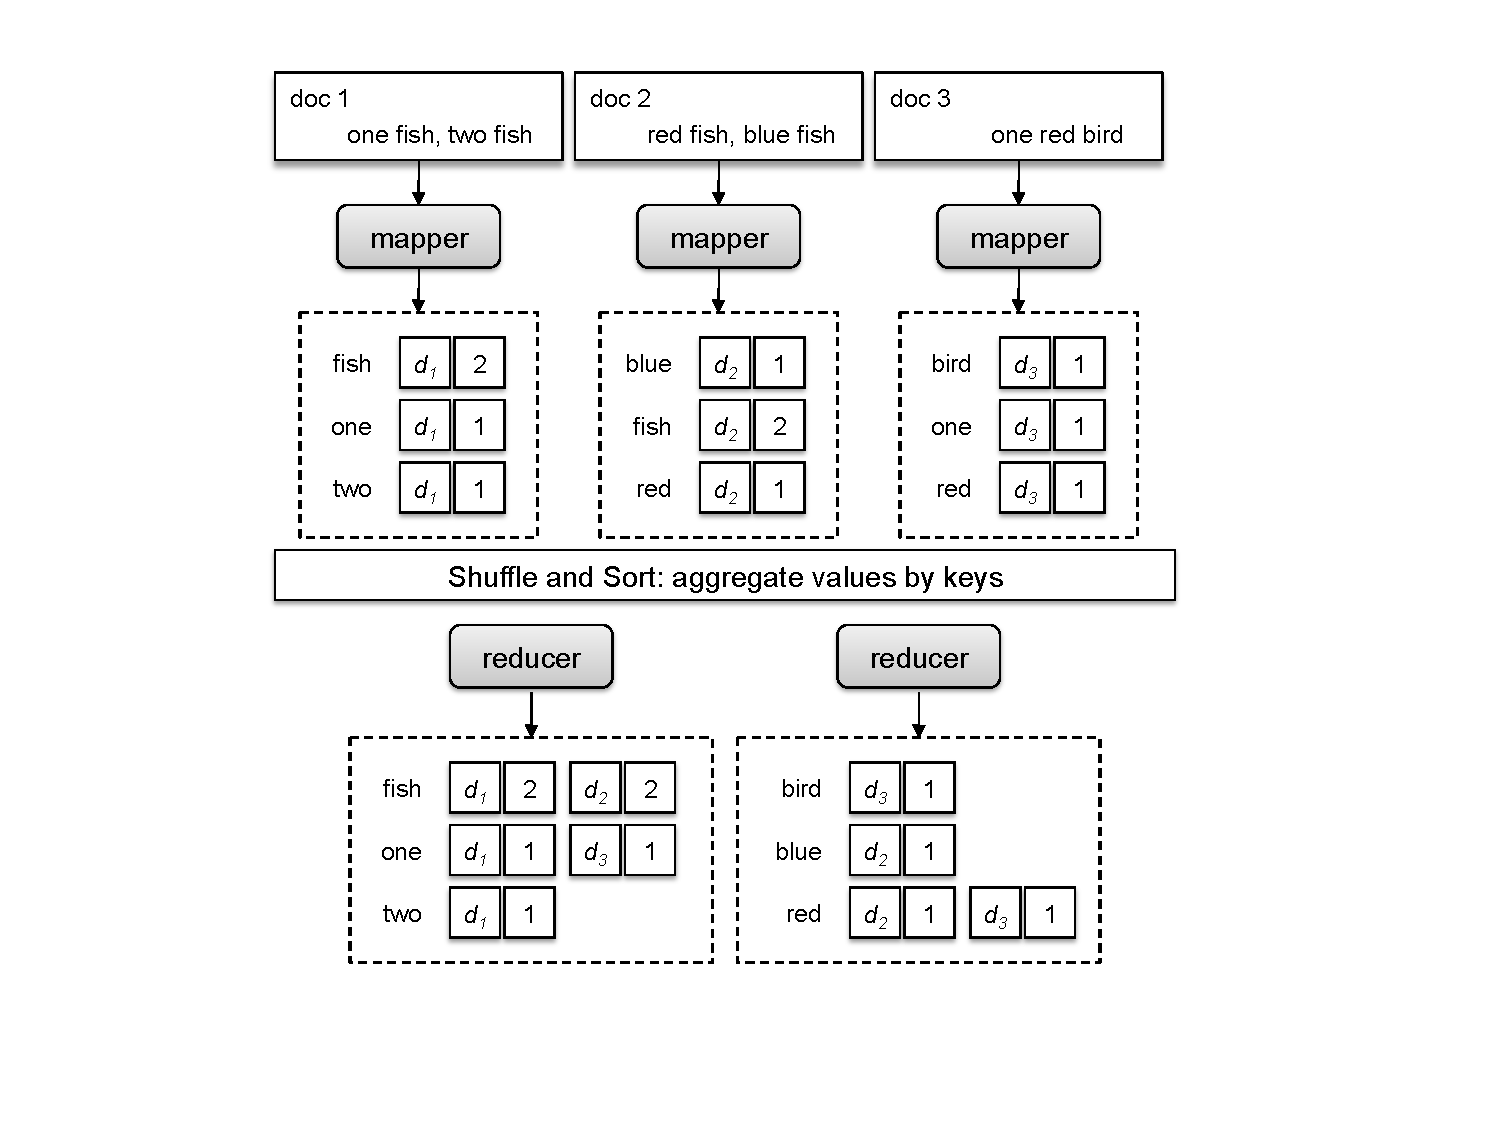
\includegraphics[scale=0.6]{figures/fig-ch4-indexing-MR-baseline.pdf}
\end{center}
\caption{Simple illustration of the baseline inverted indexing
  algorithm in MapReduce with three mappers and two reducers.
  Postings are shown as pairs of boxes (\emph{docid}, \emph{tf}).}
\label{chapter-indexing:MR-baseline}
\end{figure}

Execution of the complete algorithm is illustrated in
Figure~\ref{chapter-indexing:MR-baseline} with a toy example
consisting of three documents, three mappers, and two reducers.
Intermediate key-value pairs (from the mappers) and the final
key-value pairs comprising the inverted index (from the reducers) are
shown in the boxes with dotted lines.  Postings are shown as pairs of
boxes, with the document id on the left and the term frequency on the
right.

The MapReduce programming model provides a very concise expression of
the inverted indexing algorithm.  Its implementation is similarly
concise:\ the basic algorithm can be implemented in as few as a couple
dozen lines of code in Hadoop (with minimal document processing).
Such an implementation can be completed as a week-long programming
assignment in a course for advanced undergraduates or first-year
graduate students~\cite{KimballA_etal_2008,Lin_TeachCL2008}.  In a
non-MapReduce indexer, a significant fraction of the code is devoted
to grouping postings by term, given constraints imposed by memory and
disk (e.g., memory capacity is limited, disk seeks are slow, etc.).
In MapReduce, the programmer does not need to worry about any of these
issues---most of the heavy lifting is performed by the execution
framework.

\section{Inverted Indexing: Revised Implementation}
\label{chapter-indexing:index:revised}

The inverted indexing algorithm presented in the previous section
serves as a reasonable baseline.  However, there is a significant
scalability bottleneck:\ the algorithm assumes that there is
sufficient memory to hold all postings associated with the same term.
Since the basic MapReduce execution framework makes no guarantees
about the ordering of values associated with the same key, the reducer
first buffers all postings (line 5 of the reducer pseudo-code in
Algorithm~\ref{algorithm:chapter-indexing:indexing:basic}) and then performs an
in-memory sort before writing the postings to disk.\footnote{See
  similar discussion in Section~\ref{chapter3:secondary-sorting}:\ in
  principle, this need not be an in-memory sort.  It is entirely
  possible to implement a disk-based sort within the reducer.}  For
efficient retrieval, postings need to be sorted by document id.
However, as collections become larger, postings lists grow longer, and
at some point in time, reducers will run out of memory.

There is a simple solution to this problem.  Since the execution
framework guarantees that keys arrive at each reducer in sorted order,
one way to overcome the scalability bottleneck is to let the MapReduce
runtime do the sorting for us.  Instead of emitting key-value pairs of
the following type:

\begin{quote}
$(\textrm{term }t, \textrm{posting }\langle docid, f \rangle )$
\end{quote}

\noindent We emit intermediate key-value pairs of the type instead:

\begin{quote}
$(\textrm{tuple }\langle t, docid \rangle, \textrm{tf }f )$
\end{quote}

\noindent In other words, the key is a tuple containing the term and
the document id, while the value is the term frequency.  This is
exactly the value-to-key conversion design pattern introduced in
Section~\ref{chapter3:secondary-sorting}.  With this modification, the
programming model ensures that the postings arrive in the correct
order.  This, combined with the fact that reducers can hold state
across multiple keys, allows postings lists to be created with minimal
memory usage.  As a detail, remember that we must define a custom
partitioner to ensure that all tuples with the same term are shuffled
to the same reducer.

The revised MapReduce inverted indexing algorithm is shown in
Algorithm~\ref{algorithm:chapter-indexing:scalable}.  The mapper remains unchanged
for the most part, other than differences in the intermediate
key-value pairs.  The \textsc{Reduce} method is called for each key
(i.e., $\langle t, n \rangle$), and by design, there will only be one
value associated with each key.  For each key-value pair, a posting
can be directly added to the postings list.  Since the postings are
guaranteed to arrive in sorted order by document id, they can be
incrementally coded in compressed form---thus ensuring a small
memory footprint.  Finally, when all postings associated with the same
term have been processed (i.e., $t \ne t_{prev}$), the entire postings
list is emitted.  The final postings list must be written out in the
\textsc{Close} method.  As with the baseline algorithm, payloads can
be easily changed:\ by simply replacing the intermediate value $f$
(term frequency) with whatever else is desired (e.g., term positional
information).

\begin{algorithm}[t]
\caption{Scalable inverted indexing}
\label{algorithm:chapter-indexing:scalable}
By applying the value-to-key conversion design pattern, the execution
framework is exploited to sort postings so that they arrive sorted by
document id in the reducer.

\algrenewcommand\algorithmicfunction{\textbf{class}}
\algrenewcommand\algorithmicprocedure{\textbf{method}}
  \begin{algorithmic}[1]
    \Function{Mapper}{}
    \Procedure{Map}{$\textrm{docid }n, \textrm{doc }d$}
    \State $H \gets \textrm{new }\textsc{AssociativeArray}$
    \ForAll{$\textrm{term }t \in \textrm{doc }d$}
    \State $H\{t\} \gets H\{t\} + 1$
    \EndFor
    \ForAll{$\textrm{term }t \in H$}
    \State $\textsc{Emit}(\textrm{tuple }\langle t, n \rangle, \textrm{tf }H\{t\} )$
    \EndFor
    \EndProcedure
    \EndFunction
  \end{algorithmic}

  \begin{algorithmic}[1]
    \Function{Reducer}{}
    \Procedure{Initialize}{}
      \State $t_{prev} \gets \emptyset$
      \State $P \gets \textrm{new }\textsc{PostingsList}$
    \EndProcedure
    \Procedure{Reduce}{$\textrm{tuple }\langle t, n \rangle, \textrm{tf }[ f ]$}
    \If{$t \ne t_{prev} \land t_{prev} \ne \emptyset$}
      \State $\textsc{Emit}(\textrm{term }t_{prev}, \textrm{ postings } P)$
      \State $P.\textsc{{\small Reset}}()$
    \EndIf
    \State $P.\textsc{{\small Add}}(\langle n, f \rangle)$
    \State $t_{prev} \gets t$
    \EndProcedure
    \Procedure{Close}{}
      \State $\textsc{Emit}(\textrm{term }t, \textrm{ postings } P)$
    \EndProcedure
    \EndFunction
  \end{algorithmic}
\end{algorithm}

There is one more detail we must address when building inverted
indexes.  Since almost all retrieval models take into account document
length when computing query--document scores, this information must
also be extracted.  Although it is straightforward to express this
computation as another MapReduce job, this task can actually be folded
into the inverted indexing process.  When processing the terms in each
document, the document length is known, and can be written out as
``side data'' directly to HDFS.  We can take advantage of the ability
for a mapper to hold state across the processing of multiple documents
in the following manner:\ an in-memory associative array is created to
store document lengths, which is populated as each document is
processed.\footnote{In general, there is no worry about insufficient
  memory to hold these data.}  When the mapper finishes processing
input records, document lengths are written out to HDFS (i.e., in the
\textsc{Close} method).  This approach is essentially a variant of the
in-mapper combining pattern.  Document length data ends up in $m$
different files, where $m$ is the number of mappers; these files are
then consolidated into a more compact representation.  Alternatively,
document length information can be emitted in special key-value pairs
by the mapper.  One must then write a custom partitioner so that these
special key-value pairs are shuffled to a single reducer, which will
be responsible for writing out the length data separate from the
postings lists.

\section{Index Compression}
\label{chapter-indexing:index:compression}

We return to the question of how postings are actually compressed and
stored on disk.  This chapter devotes a substantial amount of space to
this topic because index compression is one of the main differences
between a ``toy'' indexer and one that works on real-world
collections.  Otherwise, MapReduce inverted indexing algorithms are
pretty straightforward.

Let us consider the canonical case where each posting consists of a
document id and the term frequency.  A na\"ive implementation might
represent the first as a 32-bit integer\footnote{However, note that
  $2^{32}-1$ is ``only'' 4,294,967,295, which is much less than even
  the most conservative estimate of the size of the web.} and the
second as a 16-bit integer.  Thus, a postings list might be encoded as
follows:

\begin{quote}
$[ (5, 2), (7, 3), (12, 1), (49, 1), (51, 2), \ldots]$
\end{quote}

\noindent where each posting is represented by a pair in parentheses.
Note that all brackets, parentheses, and commas are only included to
enhance readability; in reality the postings would be represented as a
long stream of integers.  This na\"ive implementation would require
six bytes per posting.  Using this scheme, the entire inverted index
would be about as large as the collection itself.  Fortunately, we can
do significantly better.

The first trick is to encode \emph{differences} between document ids as
opposed to the document ids themselves.  Since the postings are sorted
by document ids, the differences (called \emph{d}-gaps) must be
positive integers greater than zero.  The above postings list,
represented with \emph{d}-gaps, would be:

\begin{quote}
$[ (5, 2), (2, 3), (5, 1), (37, 1), (2, 2), \ldots]$
\end{quote}

\noindent Of course, we must actually encode the first document id.
We haven't lost any information, since the original document ids can
be easily reconstructed from the \emph{d}-gaps.  However, it's not
obvious that we've reduced the space requirements either, since the
largest possible \emph{d}-gap is one less than the number of documents
in the collection.

This is where the second trick comes in, which is to represent the
\emph{d}-gaps in a way such that it takes less space for smaller
numbers.  Similarly, we want to apply the same techniques to compress
the term frequencies, since for the most part they are also small
values.  But to understand how this is done, we need to take a slight
detour into compression techniques, particularly for coding integers.

Compression, in general, can be characterized as either \emph{lossless}
or \emph{lossy}:\ it's fairly obvious that loseless compression is
required in this context.  To start, it is important to understand
that all compression techniques represent a time--space tradeoff.
That is, we reduce the amount of space on disk necessary to store
data, but at the cost of extra processor cycles that must be spent
coding and decoding data.  Therefore, it is possible that compression
reduces size but also slows processing.  However, if the two factors
are properly balanced (i.e., decoding speed can keep up with disk
bandwidth), we can achieve the best of both worlds:\ smaller \emph{and}
faster.

\subsection{Byte-Aligned and Word-Aligned Codes}

In most programming languages, an integer is encoded in four bytes and
holds a value between 0 and $2^{32}-1$, inclusive. We limit our
discussion to \emph{unsigned} integers, since \emph{d}-gaps are always
positive (and greater than zero).  This means that 1 and 4,294,967,295
both occupy four bytes.  Obviously, encoding \emph{d}-gaps this way
doesn't yield any reductions in size.

A simple approach to compression is to only use as many bytes as is
necessary to represent the integer.  This is known as variable-length
integer coding (varInt for short) and accomplished by using the high
order bit of every byte as the \emph{continuation bit}, which is set to
one in the last byte and zero elsewhere.  As a result, we have 7 bits
per byte for coding the value, which means that $0 \leq n < 2^7$ can
be expressed with 1 byte, $2^{7} \leq n < 2^{14}$ with 2 bytes,
$2^{14} \leq n < 2^{21}$ with 3, and $2^{21} \leq n < 2^{28}$ with 4
bytes.  This scheme can be extended to code arbitrarily-large integers
(i.e., beyond 4 bytes).  As a concrete example, the two numbers:

\begin{quote}
127, 128
\end{quote}

\noindent would be coded as such:

\begin{quote}
1 1111111, 0 0000001 1 0000000
\end{quote}

\noindent The above code contains two code words, the first consisting
of 1 byte, and the second consisting of 2 bytes.  Of course, the comma
and the spaces are there only for readability.  Variable-length
integers are byte-aligned because the code words always fall along
byte boundaries.  As a result, there is never any ambiguity about
where one code word ends and the next begins.  However, the downside
of varInt coding is that decoding involves lots of bit operations
(masks, shifts).  Furthermore, the continuation bit sometimes results
in frequent branch mispredicts (depending on the actual distribution
of \emph{d}-gaps), which slows down processing.

A variant of the varInt scheme was described by Jeff Dean in a keynote
talk at the WSDM 2009 conference.\footnote{\texttt{
  http://research.google.com/people/jeff/WSDM09-keynote.pdf}} The
insight is to code groups of four integers at a time.  Each group
begins with a prefix byte, divided into four 2-bit values that specify
the byte length of each of the following integers.  For example, the
following prefix byte:

\begin{quote}
00,00,01,10
\end{quote}

\noindent indicates that the following four integers are one byte, one
byte, two bytes, and three bytes, respectively.  Therefore, each group
of four integers would consume anywhere between 5 and 17 bytes.  A
simple lookup table based on the prefix byte directs the decoder on
how to process subsequent bytes to recover the coded integers.  The
advantage of this group varInt coding scheme is that values can be
decoded with fewer branch mispredicts and bitwise operations.
Experiments reported by Dean suggest that decoding integers with this
scheme is more than twice as fast as the basic varInt scheme.

In most architectures, accessing entire machine words is more
efficient than fetching all its bytes separately.  Therefore, it makes
sense to store postings in increments of 16-bit, 32-bit, or 64-bit
machine words.  Anh and Moffat~\cite{Anh_Moffat_2005} presented
several word-aligned coding methods, one of which is called Simple-9,
based on 32-bit words.  In this coding scheme, four bits in each
32-bit word are reserved as a \emph{selector}.  The remaining 28 bits
are used to code actual integer values.  Now, there are a variety of
ways these 28 bits can be divided to code one or more integers:\ 28
bits can be used to code one 28-bit integer, two 14-bit integers,
three 9-bit integers (with one bit unused), etc., all the way up to
twenty-eight 1-bit integers.  In fact, there are nine different ways
the 28 bits can be divided into equal parts (hence the name of the
technique), some with leftover unused bits.  This is stored in the
selector bits.  Therefore, decoding involves reading a 32-bit word,
examining the selector to see how the remaining 28 bits are packed,
and then appropriately decoding each integer.  Coding works in the
opposite way:\ the algorithm scans ahead to see how many integers can
be squeezed into 28 bits, packs those integers, and sets the selector
bits appropriately.

\subsection{Bit-Aligned Codes}

The advantage of byte-aligned and word-aligned codes is that they can
be coded and decoded quickly.  The downside, however, is that they
\emph{must} consume multiples of eight bits, even when fewer bits might
suffice (the Simple-9 scheme gets around this by packing multiple
integers into a 32-bit word, but even then, bits are often wasted).
In bit-aligned codes, on the other hand, code words can occupy any
number of bits, meaning that boundaries can fall anywhere.  In
practice, coding and decoding bit-aligned codes require processing
bytes and appropriately shifting or masking bits (usually more
involved than varInt and group varInt coding).

One additional challenge with bit-aligned codes is that we need a
mechanism to delimit code words, i.e., tell where the last ends and
the next begins, since there are no byte boundaries to guide us.  To
address this issue, most bit-aligned codes are so-called prefix codes
(confusingly, they are also called prefix-free codes), in which no
valid code word is a prefix of any other valid code word.  For
example, coding $0 \leq x < 3$ with $\{0, 1, 01\}$ is not a valid
prefix code, since 0 is a prefix of 01, and so we can't tell if 01 is
two code words or one.  On the other hand, $\{00, 01, 1\}$ is a valid
prefix code, such that a sequence of bits:

\begin{quote}
0001101001010100
\end{quote}

\noindent can be unambiguously segmented into:

\begin{quote}
00 01 1 01 00 1 01 01 00
\end{quote}

\noindent and decoded without any additional delimiters.

One of the simplest prefix codes is the unary code.  An integer $x>0$
is coded as $x-1$ one bits followed by a zero bit.  Note that unary
codes do not allow the representation of zero, which is fine since
\emph{d}-gaps and term frequencies should never be zero.\footnote{As a
  note, some sources describe slightly different formulations of the
  same coding scheme.  Here, we adopt the conventions used in the
  classic IR text \emph{Managing Gigabytes}~\cite{Witten_etal_1999}.}
As an example, 4 in unary code is 1110.  With unary code we can code
$x$ in $x$ bits, which although economical for small values, becomes
inefficient for even moderately large values.  Unary codes are rarely
used by themselves, but form a component of other coding schemes.
Unary codes of the first ten positive integers are shown in
Figure~\ref{chapter-indexing:encoding-schemes}.

\begin{figure}[t]
\centering
\begin{tabular}{lllll}
\hline
    &       &          & Golomb \\
$x$ & unary & $\gamma$ & $b=5$ & $b=10$\\
\hline
1  & 0          & 0        & 0:00   & 0:000\\
2  & 10         & 10:0     & 0:01   & 0:001\\
3  & 110        & 10:1     & 0:10   & 0:010\\
4  & 1110       & 110:00   & 0:110  & 0:011\\
5  & 11110      & 110:01   & 0:111  & 0:100\\
6  & 111110     & 110:10   & 10:00  & 0:101\\
7  & 1111110    & 110:11   & 10:01  & 0:1100\\
8  & 11111110   & 1110:000 & 10:10  & 0:1101\\
9  & 111111110  & 1110:001 & 10:110 & 0:1110\\
10 & 1111111110 & 1110:010 & 10:111 & 0:1111\\
\hline
\end{tabular}
\caption{The first ten positive integers in unary, $\gamma$, and
  Golomb ($b=5,10$) codes.}
\label{chapter-indexing:encoding-schemes}
\end{figure}

Elias $\gamma$ code is an efficient coding scheme that is widely used
in practice.  An integer $x>0$ is broken into two components, $1 +
\lfloor \log_2 x \rfloor$ ($=n$, the length), which is coded in unary
code, and $x-2^{\lfloor \log_2 x \rfloor}$ ($=r$, the remainder),
which is in binary.\footnote{Note that $\lfloor x \rfloor$ is the
  floor function, which maps $x$ to the largest integer not greater
  than $x$, so, e.g., $\lfloor 3.8 \rfloor = 3$. This is the default
  behavior in many programming languages when casting from a
  floating-point type to an integer type.}  The unary component $n$
specifies the number of bits required to code $x$, and the binary
component codes the remainder $r$ in $n-1$ bits.  As an example,
consider $x=10$: $1 + \lfloor \log_2 10 \rfloor = 4$, which is 1110.
The binary component codes $x-2^3=2$ in $4-1=3$ bits, which is 010.
Putting both together, we arrive at 1110:010. The extra colon is
inserted only for readability; it's not part of the final code, of
course.

Working in reverse, it is easy to unambiguously decode a bit stream of
$\gamma$ codes: First, we read a unary code $c_u$, which is a prefix
code.  This tells us that the binary portion is written in $c_u-1$
bits, which we then read as $c_b$.  We can then reconstruct $x$ as
$2^{c_u-1} + c_b$.  For $x<16$, $\gamma$ codes occupy less than a full
byte, which makes them more compact than variable-length integer
codes.  Since term frequencies for the most part are relatively small,
$\gamma$ codes make sense for them and can yield substantial space
savings.  For reference, the $\gamma$ codes of the first ten positive
integers are shown in Figure~\ref{chapter-indexing:encoding-schemes}.
A variation on $\gamma$ code is $\delta$ code, where the $n$ portion
of the $\gamma$ code is coded in $\gamma$ code itself (as opposed to
unary code).  For smaller values $\gamma$ codes are more compact, but
for larger values, $\delta$ codes take less space.

Unary and $\gamma$ codes are parameterless, but even better
compression can be achieved with parameterized codes.  A good example
of this is Golomb code.  For some parameter $b$, an integer $x>0$ is
coded in two parts:\ first, we compute $q = \lfloor (x-1)/b \rfloor$
and code $q+1$ in unary; then, we code the remainder $r = x - qb -1$
in truncated binary.  This is accomplished as follows:\ if $b$ is a
power of two, then truncated binary is exactly the same as normal
binary, requiring $\log_2 b$ bits.  Otherwise, we code the first
$2^{\lfloor \log_2 b \rfloor+1} - b$ values of $r$ in $\lfloor \log_2
b \rfloor$ bits and code the rest of the values of $r$ by coding
$r+2^{\lfloor \log_2 b \rfloor+1} - b$ in ordinary binary
representation using $\lfloor \log_2 b \rfloor+1$ bits.  In this case,
the $r$ is coded in either $\lfloor \log_2 b \rfloor$ or $\lfloor
\log_2 b \rfloor +1$ bits, and unlike ordinary binary coding,
truncated binary codes are prefix codes.  As an example, if $b=5$,
then $r$ can take the values $\{0, 1, 2, 3, 4\}$, which would be coded
with the following code words: $\{00,01,10,110,111\}$.  For reference,
Golomb codes of the first ten positive integers are shown in
Figure~\ref{chapter-indexing:encoding-schemes} for $b=5$ and $b=10$.
A special case of Golomb code is worth noting:\ if $b$ is a power of
two, then coding and decoding can be handled more efficiently (needing
only bit shifts and bit masks, as opposed to multiplication and
division).  These are known as Rice codes.

Researchers have shown that Golomb compression works well for \emph{
  d}-gaps, and is optimal with the following parameter setting:

\begin{equation}
b \approx 0.69 \times \frac{df}{N}
\end{equation}

\noindent where $df$ is the document frequency of the term, and $N$ is
the number of documents in the collection.\footnote{For details as to
  why this is the case, we refer the reader
  elsewhere~\cite{Witten_etal_1999}, but here's the intuition:\ under
  reasonable assumptions, the appearance of postings can be modeled as
  a sequence of independent Bernoulli trials, which implies a certain
  distribution of \emph{d}-gaps.  From this we can derive an optimal
  setting of $b$.}

Putting everything together, one popular approach for postings
compression is to represent \emph{d}-gaps with Golomb codes and term
frequencies with $\gamma$
codes~\cite{Witten_etal_1999,Zobel_Moffat_2006}.  If positional
information is desired, we can use the same trick to code differences
between term positions using $\gamma$ codes.

\subsection{Postings Compression}

Having completed our slight detour into integer compression
techniques, we can now return to the scalable inverted indexing
algorithm shown in Algorithm~\ref{algorithm:chapter-indexing:scalable} and discuss
how postings lists can be properly compressed.  As we can see from the
previous section, there is a wide range of choices that represent
different tradeoffs between compression ratio and decoding speed.
Actual performance also depends on characteristics of the collection,
which, among other factors, determine the distribution of \emph{
  d}-gaps.  B\"uttcher et al.~\cite{Buttcher_etal_2010} recently
compared the performance of various compression techniques on coding
document ids.  In terms of the amount of compression that can be
obtained (measured in bits per \emph{docid}), Golomb and Rice codes
performed the best, followed by $\gamma$ codes, Simple-9, varInt, and
group varInt (the least space efficient).  In terms of raw decoding
speed, the order was almost the reverse:\ group varInt was the
fastest, followed by varInt.\footnote{However, this study found less
  speed difference between group varInt and basic varInt than Dean's
  analysis, presumably due to the different distribution of \emph{d}-gaps
  in the collections they were examining.}  Simple-9 was substantially
slower, and the bit-aligned codes were even slower than that.  Within
the bit-aligned codes, Rice codes were the fastest, followed by
$\gamma$, with Golomb codes being the slowest (about ten times slower
than group varInt).

Let us discuss what modifications are necessary to our inverted
indexing algorithm if we were to adopt Golomb compression for \emph{
  d}-gaps and represent term frequencies with $\gamma$ codes.  Note
that this represents a space-efficient encoding, at the cost of slower
decoding compared to alternatives.  Whether or not this is actually a
worthwhile tradeoff in practice is not important here:\ use of Golomb
codes serves a pedagogical purpose, to illustrate how one might set
compression parameters.

Coding term frequencies with $\gamma$ codes is easy since they are
parameterless.  Compressing \emph{d}-gaps with Golomb codes, however,
is a bit tricky, since two parameters are required:\ the size of the
document collection and the number of postings for a particular
postings list (i.e., the document frequency, or \emph{df}).  The first
is easy to obtain and can be passed into the reducer as a constant.
The \emph{df} of a term, however, is not known until all the postings
have been processed---and unfortunately, the parameter must be known
before any posting is coded.  At first glance, this seems like a
chicken-and-egg problem.  A two-pass solution that involves first
buffering the postings (in memory) would suffer from the memory
bottleneck we've been trying to avoid in the first place.

To get around this problem, we need to somehow inform the reducer of a
term's \emph{df} before any of its postings arrive.  This can be solved
with the order inversion design pattern introduced in
Section~\ref{chapter3:cond-prob} to compute relative frequencies.  The
solution is to have the mapper emit special keys of the form $\langle
t, \ast \rangle$ to communicate partial document frequencies.  That
is, inside the mapper, in addition to emitting intermediate key-value
pairs of the following form:

\begin{quote}
$(\textrm{tuple }\langle t, docid \rangle, \textrm{tf }f )$
\end{quote}

\noindent we also emit special intermediate key-value pairs like this:

\begin{quote}
$(\textrm{tuple }\langle t, \ast \rangle, \textrm{df }e )$
\end{quote}

\noindent to keep track of document frequencies associated with each
term.  In practice, we can accomplish this by applying the in-mapper
combining design pattern (see
Section~\ref{chapter3:local-aggregation}).  The mapper holds an
in-memory associative array that keeps track of how many documents a
term has been observed in (i.e., the local document frequency of the
term for the subset of documents processed by the mapper).  Once the
mapper has processed all input records, special keys of the form
$\langle t, \ast \rangle$ are emitted with the partial \emph{df} as the
value.

To ensure that these special keys arrive first, we define the sort
order of the tuple so that the special symbol $\ast$ precedes all
documents (part of the order inversion design pattern).  Thus, for
each term, the reducer will first encounter the $\langle t, \ast
\rangle$ key, associated with a list of values representing partial
       \emph{df} values originating from each mapper.  Summing all
       these partial contributions will yield the term's \emph{df},
       which can then be used to set the Golomb compression parameter
       $b$.  This allows the postings to be incrementally compressed
       as they are encountered in the reducer---memory bottlenecks are
       eliminated since we do not need to buffer postings in memory.

Once again, the order inversion design pattern comes to the rescue.
Recall that the pattern is useful when a reducer needs to access the
result of a computation (e.g., an aggregate statistic) before it
encounters the data necessary to produce that computation.  For
computing relative frequencies, that bit of information was the
marginal.  In this case, it's the document frequency.

\section{What About Retrieval?}
\label{chapter-indexing:retrieval}

Thus far, we have briefly discussed web crawling and focused mostly on
MapReduce algorithms for inverted indexing.  What about retrieval?  It
should be fairly obvious that MapReduce, which was designed for large
batch operations, is a poor solution for retrieval.  Since users
demand sub-second response times, every aspect of retrieval must be
optimized for low latency, which is exactly the opposite tradeoff made
in MapReduce.  Recall the basic retrieval problem:\ we must look up
postings lists corresponding to query terms, systematically traverse
those postings lists to compute query--document scores, and then
return the top $k$ results to the user.  Looking up postings implies
random disk seeks, since for the most part postings are too large to
fit into memory (leaving aside caching and other special cases for
now).  Unfortunately, random access is not a forte of the distributed
file system underlying MapReduce---such operations require multiple
round-trip network exchanges (and associated latencies).  In HDFS, a
client must first obtain the location of the desired data block from
the namenode before the appropriate datanode can be contacted for the
actual data.  Of course, access will typically require a random disk
seek on the datanode itself.

It should be fairly obvious that serving the search needs of a large
number of users, each of whom demand sub-second response times, is
beyond the capabilities of any single machine.  The only solution is
to distribute retrieval across a large number of machines, which
necessitates breaking up the index in some manner.  There are two main
partitioning strategies for distributed retrieval:\ \emph{document
  partitioning} and \emph{term partitioning}.  Under document
partitioning, the entire collection is broken up into multiple smaller
sub-collections, each of which is assigned to a server.  In other
words, each server holds the complete index for a subset of the entire
collection.  This corresponds to partitioning vertically in
Figure~\ref{chapter-indexing:partition}.  With term partitioning, on
the other hand, each server is responsible for a subset of the terms
for the entire collection.  That is, a server holds the postings for
all documents in the collection for a subset of terms.  This
corresponds to partitioning horizontally in
Figure~\ref{chapter-indexing:partition}.

\begin{figure}[t]
\begin{center}
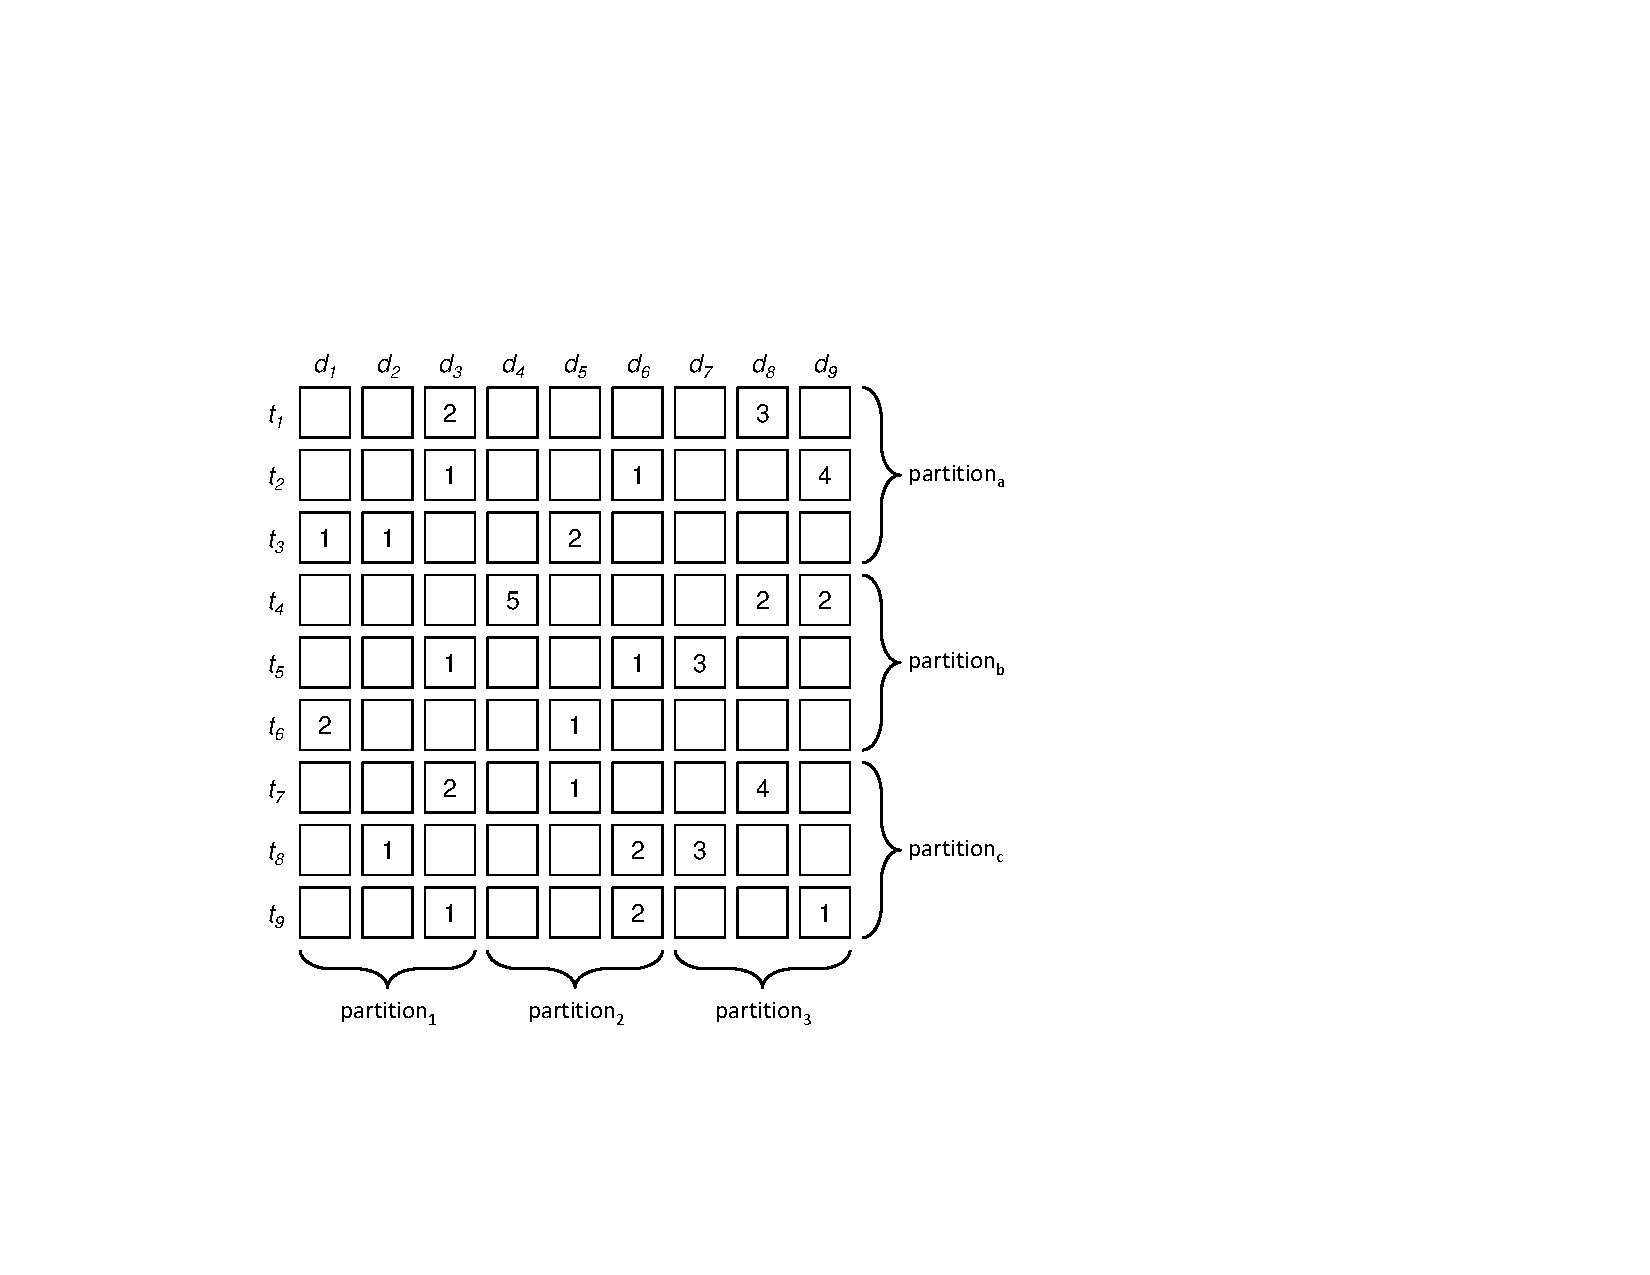
\includegraphics[scale=0.75]{figures/fig-ch4-indexing-partition.pdf}
\end{center}
\caption{Term--document matrix for a toy collection (nine documents,
  nine terms) illustrating different partitioning
  strategies:\ partitioning vertically ($1,2,3$) corresponds to
  document partitioning, whereas partitioning horizontally ($a,b,c$)
  corresponds to term partitioning.}
\label{chapter-indexing:partition}
\end{figure}

Document and term partitioning require different retrieval strategies
and represent different tradeoffs.  Retrieval under document
partitioning involves a query broker, which forwards the user's query
to all partition servers, merges partial results from each, and then
returns the final results to the user.  With this architecture,
searching the entire collection requires that the query be processed
by every partition server.  However, since each partition operates
independently and traverses postings in parallel, document
partitioning typically yields shorter query latencies (compared to a
single monolithic index with much longer postings lists).  

Retrieval under term partitioning, on the other hand, requires a very
different strategy.  Suppose the user's query $Q$ contains three
terms, $q_1$, $q_2$, and $q_3$.  Under the pipelined query evaluation
strategy, the broker begins by forwarding the query to the server that
holds the postings for $q_1$ (usually the least frequent term).  The
server traverses the appropriate postings list and computes partial
query--document scores, stored in the accumulators.  The accumulators
are then passed to the server that holds the postings associated with
$q_2$ for additional processing, and then to the server for $q_3$,
before final results are passed back to the broker and returned to the
user.  Although this query evaluation strategy may not substantially
reduce the latency of any particular query, it can theoretically
increase a system's throughput due to the far smaller number of total
disk seeks required for each user query (compared to document
partitioning).  However, load-balancing is tricky in a pipelined
term-partitioned architecture due to skew in the distribution of query
terms, which can create ``hot spots'' on servers that hold the
postings for frequently-occurring query terms.

In general, studies have shown that document partitioning is a better
strategy overall~\cite{Moffat_etal_SIGIR2006}, and this is the
strategy adopted by Google~\cite{Barroso03}.  Furthermore, it is known
that Google maintains its indexes in memory (although this is
certainly not the common case for search engines in general).  One key
advantage of document partitioning is that result quality degrades
gracefully with machine failures.  Partition servers that are offline
will simply fail to deliver results for their subsets of the
collection.  With sufficient partitions, users might not even be aware
that documents are missing.  For most queries, the web contains
more relevant documents than any user has time to digest:\ users of
course care about getting relevant documents (sometimes, they are
happy with a single relevant document), but they are generally less
discriminating when it comes to \emph{which} relevant documents appear
in their results (out of the set of \emph{all} relevant documents).
Note that partitions may be unavailable due to reasons other than
machine failure:\ cycling through different partitions is a very
simple and non-disruptive strategy for index updates.

Working in a document-partitioned architecture, there are a variety of
approaches to dividing up the web into smaller pieces.  Proper
partitioning of the collection can address one major weakness of this
architecture, which is that every partition server is involved in
every user query.  Along one dimension, it is desirable to partition
by document quality using one or more classifiers; see~\cite{qiACS09}
for a recent survey on web page classification.  Partitioning by
document quality supports a multi-phase search strategy:\ the system
examines partitions containing high quality documents first, and only
backs off to partitions containing lower quality documents if
necessary.  This reduces the number of servers that need to be
contacted for a user query.  Along an orthogonal dimension, it is
desirable to partition documents by content (perhaps also guided by
the distribution of user queries from logs), so that each partition is
``well separated'' from the others in terms of topical
coverage.  This also reduces the number of machines that need
to be involved in serving a user's query:\ the broker can direct
queries only to the partitions that are likely to contain relevant
documents, as opposed to forwarding the user query to all the
partitions.

On a large-scale, reliability of service is provided by replication,
both in terms of multiple machines serving the same partition within a
single datacenter, but also replication across
geographically-distributed datacenters.  This creates at least two
query routing problems:\ since it makes sense to serve clients from
the closest datacenter, a service must route queries to the
appropriate location.  Within a single datacenter, the system needs to
properly balance load across replicas.

There are two final components of real-world search engines that are
worth discussing.  First, recall that postings only store document
ids.  Therefore, raw retrieval results consist of a ranked list of
semantically meaningless document ids.  It is typically the
responsibility of document servers, functionally distinct from the
partition servers holding the indexes, to generate meaningful output
for user presentation.  Abstractly, a document server takes as
input a query and a document id, and computes an appropriate result
entry, typically comprising the title and URL of the page, a snippet
of the source document showing the user's query terms in context, and
additional metadata about the document.  Second, query evaluation can
benefit immensely from caching, of individual postings (assuming that
the index is not already in memory) and even results of entire
queries~\cite{Baeza-Yates_etal_SIGIR2007}.  This is made possible by
the Zipfian distribution of queries, with very frequent queries at the
head of the distribution dominating the total number of queries.
Search engines take advantage of this with cache servers, which are
functionally distinct from all of the components discussed above.

\section{Summary and Additional Readings}
\label{chapter-indexing:summary}

Web search is a complex problem that breaks down into three
conceptually-distinct components.  First, the documents collection
must be gathered (by crawling the web).  Next, inverted indexes and
other auxiliary data structures must be built from the documents.
Both of these can be considered offline problems.  Finally, index
structures must be accessed and processed in response to user queries
to generate search results.  This last task is an online problem that
demands both low latency and high throughput.

This chapter primarily focused on building inverted indexes, the
problem most suitable for MapReduce.  After all, inverted indexing is
nothing but a very large distributed sort and group by operation!  We
began with a baseline implementation of an inverted indexing
algorithm, but quickly noticed a scalability bottleneck that stemmed
from having to buffer postings in memory.  Application of the
value-to-key conversion design pattern
(Section~\ref{chapter3:secondary-sorting}) addressed the issue by
offloading the task of sorting postings by document id to the
MapReduce execution framework.  We also surveyed various techniques
for integer compression, which yield postings lists that are both more
compact and faster to process.  As a specific example, one could use
Golomb codes for compressing \emph{d}-gaps and $\gamma$ codes for term
frequencies.  We showed how the order inversion design pattern
introduced in Section~\ref{chapter3:cond-prob} for computing relative
frequencies can be used to properly set compression parameters.

\paragraph{Additional Readings.} 
Our brief discussion of web search glosses over many complexities and
does a huge injustice to the tremendous amount of research in
information retrieval.  Here, however, we provide a few entry points
into the literature.  A survey article by Zobel and
Moffat~\cite{Zobel_Moffat_2006} is an excellent starting point on
indexing and retrieval algorithms.  Another by Baeza-Yates et
al.~\cite{Baeza-Yates_etal_2007} overviews many important issues in
distributed retrieval.  A keynote talk at the WSDM 2009 conference by
Jeff Dean revealed a lot of information about the evolution of the
Google search architecture.\footnote{\texttt{
  http://research.google.com/people/jeff/WSDM09-keynote.pdf}} Finally,
a number of general information retrieval textbooks have been recently
published~\cite{Manning_etal_2008,Croft_etal_2009,Buttcher_etal_2010}.
Of these three, the one by B\"uttcher et al.~\cite{Buttcher_etal_2010}
is noteworthy in having detailed experimental evaluations that compare
the performance (both effectiveness and efficiency) of a wide range of
algorithms and techniques.  While outdated in many other respects, the
textbook \emph{Managing Gigabytes}~\cite{Witten_etal_1999} remains an
excellent source for index compression techniques.  Finally, ACM SIGIR
is an annual conference and the most prestigious venue for academic
information retrieval research; proceedings from those events are
perhaps the best starting point for those wishing to keep abreast of
publicly-documented developments in the field.
